\documentclass[12pt,a4paper]{ctexart}

% ========== 页面与字体 ==========
\usepackage{geometry}
\geometry{left=2.6cm,right=2.6cm,top=2.5cm,bottom=2.5cm}

\usepackage{fontspec}
\setmainfont{Times New Roman}
\IfFontExistsTF{Consolas}
  {\setmonofont{Consolas}}
  {\setmonofont{Courier New}}

\usepackage{setspace}
\onehalfspacing

% ========== 数学与图表 ==========
\usepackage{amsmath, amsthm}
\usepackage{unicode-math}
\IfFontExistsTF{Cambria Math}{\setmathfont{Cambria Math}}{}
\usepackage{graphicx}
\usepackage{booktabs}
\usepackage{array}
\usepackage{caption}
\usepackage{subcaption}
\graphicspath{{figures/}}
\captionsetup{font=small,labelfont=bf}

% ========== 颜色与链接 ==========
\usepackage{xcolor}
\definecolor{mainblue}{HTML}{2F5597}
\definecolor{lightblue}{HTML}{EAF2FF}
\definecolor{darkgray}{HTML}{333333}

\usepackage[
    colorlinks=true,
    linkcolor=mainblue,
    citecolor=mainblue,
    urlcolor=mainblue
]{hyperref}

% ========== 标题样式 ==========
\usepackage{titlesec}

\titleformat{\section}
  {\Large\bfseries\color{mainblue}}
  {\thesection}{0.8em}{}

\titleformat{\subsection}
  {\large\bfseries\color{darkgray}}
  {\thesubsection}{0.8em}{}

\titleformat{\subsubsection}
  {\normalsize\bfseries}
  {\thesubsubsection}{0.8em}{}

% ========== 页眉页脚 ==========
\usepackage{fancyhdr}
\pagestyle{fancy}
\setlength{\headheight}{14.5pt}
\fancyhf{}
\fancyhead[L]{\color{mainblue}髋膝关节跟踪控制方法研究}
\fancyhead[R]{\color{mainblue}\leftmark}
\fancyfoot[C]{\thepage}

\renewcommand{\headrulewidth}{0.4pt}
\renewcommand{\footrulewidth}{0pt}

% ========== 代码样式 ==========
\usepackage{listings}

\lstset{
    basicstyle=\ttfamily\small,
    keywordstyle=\color{mainblue}\bfseries,
    commentstyle=\color{gray},
    stringstyle=\color{teal},
    numbers=left,
    numberstyle=\tiny\color{gray},
    frame=single,
    breaklines=true,
    backgroundcolor=\color{lightblue},
    rulecolor=\color{mainblue},
    tabsize=4
}

% ========== 漂亮的提示框 ==========
\usepackage[most]{tcolorbox}

\newtcolorbox{notebox}{
    colback=lightblue,
    colframe=mainblue,
    arc=2mm,
    boxrule=0.8pt,
    left=8pt,
    right=8pt,
    top=6pt,
    bottom=6pt,
    title=\textbf{提示}
}

% ========== 定理环境 ==========
\newtheorem{theorem}{定理}
\newtheorem{definition}{定义}
\newtheorem{example}{例}

% ========== 文档信息 ==========
\title{
    \vspace{2cm}
    \Huge \textbf{\color{mainblue}基于预览 MPC 与输入域 EID 的髋膝关节跟踪控制方法研究} \\[0.5em]
    \Large Reference Generation and Input-Domain Disturbance Compensation for Hip--Knee Tracking Control
}
\author{
    技术报告
}
\date{2026年7月}

\begin{document}

\maketitle
\thispagestyle{empty}

\vspace{1.2cm}

\begin{abstract}
本文围绕右髋俯仰关节与右膝关节的周期跟踪控制问题，整理并贯通两条当前保留的方法线：其一是在参考生成层使用基于 jerk 决策变量的软预览 MPC，并进一步考察四点速度预览变体；其二是在输入补偿层分析 EID 观测量从状态域到力矩域的输入逆映射。两者分别作用于闭环系统的不同位置。预览 MPC 决定控制器所跟踪的平滑参考轨迹，输入域 EID 决定未建模动态和扰动如何以力矩补偿的形式进入执行端。本文先给出三点软预览 MPC 的线性预测模型、目标函数和等式约束，再推导四点速度预览变体的附加速度软约束；随后从当前半隐式欧拉单关节模型出发，推导输入矩阵及其 Moore--Penrose 伪逆，并说明输入逆等效增益与原经验增益之间的数量关系。实验结果表明，四点速度预览在 MuJoCo 中主要改善策略点速度一致性，位置跟踪误差几乎不变；普通伪逆输入补偿在 MuJoCo 中未导致发散，但会显著放大速度残差对应的力矩补偿。本文据此呈现方法推导、数值尺度和实验现象，不进一步给出实机替换形式。
\end{abstract}

\vspace{0.5cm}
\noindent\textbf{关键词：}预览 MPC；EID；输入逆；髋膝关节；扰动补偿；MuJoCo

\newpage
\tableofcontents
\newpage

\section{引言}

髋膝关节的周期跟踪控制同时受到两类问题制约。第一类问题发生在参考生成层：策略侧通常只给出较稀疏的位置节点，而低层控制以更高频率运行，因此需要在策略节点之间生成连续、平滑且可执行的参考位置、速度和加速度。第二类问题发生在输入补偿层：即使参考轨迹足够平滑，单关节局部模型仍会受到摩擦、重力拟合误差、耦合动态和执行端偏差的影响；这些误差若不能被合理补偿，就会表现为持续的跟踪偏差或额外的力矩振荡。

本文将这两类问题放在同一闭环框架下讨论。预览 MPC 负责把离散策略节点转化为控制周期上的参考序列，它的设计重点是位置到达、速度连续性、加速度和 jerk 平滑性之间的折中。EID 负责在控制端估计等效扰动并形成输入补偿，它的设计重点是如何把状态域估计量转换为力矩域补偿量。两者的作用层次不同，不能互相替代，但它们共同决定闭环系统在跟踪误差、力矩平滑性和鲁棒性之间的实际折中。

本文的证据边界是明确的。预览 MPC 的四点速度预览变体只在 MuJoCo 闭环仿真中与三点软预览基线进行比较；EID 输入逆部分包含离线重放、MuJoCo 等效增益闭环对比以及当前实机控制器的基准误差。本文不声称二者已经形成一个完整的新实机默认控制器，也不在此给出普通伪逆补偿的实机替换方案。相反，本文的目标是把方法推导、数值大小和实验现象整理为后续闭环设计的依据。

\section{闭环结构与问题分解}

当前控制框架可以从参考生成和输入补偿两个层面理解。参考生成层接收策略周期上的位置节点，并在控制周期上输出参考位置、速度和加速度。控制器随后根据参考状态、当前状态以及 EID 估计量计算力矩命令。若记真实状态为
\[
    x_k=\begin{bmatrix}q_k & \dot q_k\end{bmatrix}^T,
\]
观测器内部的名义状态为 \(\hat x_k\)，EID 状态修正量为 \(\eta_k\)，则反馈中心状态可以写为
\[
    \bar x_k=\hat x_k+\eta_k.
\]
在原始 EID 控制结构中，名义逆模型给出前馈力矩 \(u_k^\star\)，状态修正量经经验输入映射形成力矩补偿
\[
    \eta_{u,k}=K_u\eta_k,
\]
最终控制律可以概括为
\[
    u_k=u_k^\star-\eta_{u,k}+K(r_k-\bar x_k),
\]
其中 \(r_k\) 为参考状态，\(K\) 为反馈增益。EID 更新则利用真实状态与反馈中心状态之间的残差：
\[
    \eta_{k+1}=\alpha K_o(x_k-\bar x_k)+(1-\alpha)\eta_k .
\]
这一结构的关键特点是，EID 首先在状态域形成修正，再通过某个输入映射进入力矩域。原控制器使用固定经验增益 \(K_u=(12,1)\)，而输入逆分析试图回答的问题是：若严格依据当前离散单关节模型的输入矩阵，状态域残差应当如何映射到输入力矩域。

\section{预览 MPC 参考生成}

\subsection{三点软预览模型}

设策略周期为 \(T_p\)，控制周期为 \(dt\)，一个策略周期包含
\[
    N_p=\mathrm{round}(T_p/dt)
\]
个控制步。三点软预览 MPC 在一个滚动窗口内使用三个策略位置节点
\[
    q_0^\ast,\quad q_1^\ast,\quad q_2^\ast,
\]
预测窗口长度为 \(N_h=3N_p\)。每个关节的参考状态取为
\[
    x_k=\begin{bmatrix}q_k & \dot q_k & \ddot q_k\end{bmatrix}^T,
\]
决策变量为控制周期上的 jerk 序列
\[
    J=\begin{bmatrix}j_0 & j_1 & \cdots & j_{N_h-1}\end{bmatrix}^T .
\]
在每个控制步内假设 jerk 为常值，则离散积分关系为
\[
    \ddot q_{k+1}=\ddot q_k+dt\,j_k,
\]
\[
    \dot q_{k+1}=\dot q_k+dt\,\ddot q_k+\frac{1}{2}dt^2j_k,
\]
\[
    q_{k+1}=q_k+dt\,\dot q_k+\frac{1}{2}dt^2\ddot q_k+\frac{1}{6}dt^3j_k.
\]
由于上述预测对 \(J\) 是线性的，整个窗口可以写为
\[
    q=q_b+A_qJ,\qquad
    \dot q=\dot q_b+A_vJ,\qquad
    \ddot q=\ddot q_b+A_aJ.
\]
其中 \(q_b,\dot q_b,\ddot q_b\) 表示从当前初始状态出发且未来 jerk 为零时的基线轨迹，\(A_q,A_v,A_a\) 为由积分关系确定的下三角响应矩阵。

三点软预览方法的目标函数同时考虑参考速度、参考加速度、jerk 正则化和后两个策略点的位置贴合：
\[
\begin{aligned}
\min_J\quad
&\sum_{k=1}^{N_h}\left(w_v\dot q_k^2+w_a\ddot q_k^2\right)
 + w_j\sum_{i=0}^{N_h-1}j_i^2 \\
&+w_p\left[
(q_{2N_p}-q_1^\ast)^2+
(q_{3N_p}-q_2^\ast)^2
\right]
 +w_r\sum_{i=0}^{N_h-1}j_i^2 .
\end{aligned}
\]
第一个策略点采用硬约束
\[
    q_{N_p}=q_0^\ast,
\]
后两个策略点以软约束形式进入目标函数。这样做的意义在于，当前即将执行的策略周期必须到达第一个节点，而更远端节点只用于提供预览趋势，避免远端边界条件过硬导致参考加速度或 jerk 被动放大。

代入线性预测关系后，问题成为等式约束二次规划
\[
    \min_J \frac{1}{2}J^THJ+g^TJ,\qquad CJ=d,
\]
其中
\[
    C=A_q(N_p,:),\qquad d=q_0^\ast-q_b(N_p).
\]
KKT 系统为
\[
\begin{bmatrix}
H & C^T\\
C & 0
\end{bmatrix}
\begin{bmatrix}
J\\
\lambda
\end{bmatrix}
=
\begin{bmatrix}
-g\\
d
\end{bmatrix}.
\]
求解后只执行第一个策略周期内的参考序列，并在下一个策略周期重新滚动求解。

\subsection{四点速度预览变体}

四点速度预览变体保留上述状态、决策变量、窗口长度、硬约束和原有软预览目标。它额外使用第四个策略位置节点
\[
    q_0^\ast,\quad q_1^\ast,\quad q_2^\ast,\quad q_3^\ast,
\]
通过相邻策略位置差分构造前三个策略区间的速度目标：
\[
    v_i^\ast=\frac{q_{i+1}^\ast-q_i^\ast}{T_p},\qquad i=0,1,2.
\]
令
\[
    m_i=(i+1)N_p,\qquad i=0,1,2,
\]
表示三个策略周期末端在预测窗口中的采样行，并定义
\[
    a_{q,i}^T=A_q(m_i,:),\qquad a_{v,i}^T=A_v(m_i,:).
\]
则策略周期末端的位置与速度预测为
\[
    q_{m_i}=q_{b,m_i}+a_{q,i}^TJ,\qquad
    \dot q_{m_i}=\dot q_{b,m_i}+a_{v,i}^TJ .
\]
新增速度软预览项为
\[
    w_{pv}\sum_{i=0}^{2}\left(\dot q_{m_i}-v_i^\ast\right)^2 .
\]
因此完整目标函数可写为
\[
\begin{aligned}
\min_J\quad
&\sum_{k=1}^{N_h}\left(w_v\dot q_k^2+w_a\ddot q_k^2\right)
 +w_j\sum_{i=0}^{N_h-1}j_i^2\\
&+w_p\left[
\left(q_{2N_p}-q_1^\ast\right)^2+
\left(q_{3N_p}-q_2^\ast\right)^2
\right]\\
&+w_{pv}\sum_{i=0}^{2}
\left(\dot q_{m_i}-v_i^\ast\right)^2
 +w_r\sum_{i=0}^{N_h-1}j_i^2 .
\end{aligned}
\]
在矩阵形式中，新增项对 Hessian 和线性项的贡献分别为
\[
    H_{\dot q}=w_{pv}\sum_{i=0}^{2}a_{v,i}a_{v,i}^T,
\]
\[
    g_{\dot q}=w_{pv}\sum_{i=0}^{2}a_{v,i}
    \left(\dot q_{b,m_i}-v_i^\ast\right).
\]
当前权重设置见表~\ref{tab:mpc_weights}。其中速度预览权重保持为较小的软约束，目的不是把速度目标做成硬边界，而是让策略节点之间隐含的速度趋势温和地参与优化。

\begin{table}[htbp]
\centering
\caption{预览 MPC 目标函数权重}
\label{tab:mpc_weights}
\begin{tabular}{cccc}
\toprule
符号 & 数值 & 作用 & 适用方法 \\
\midrule
\(w_p\) & \(2.0\times10^{7}\) & 后两个策略点位置软预览 & 三点与四点 \\
\(w_v\) & \(3.0\times10^{-3}\) & 参考速度抑制 & 三点与四点 \\
\(w_a\) & \(8.0\times10^{-5}\) & 参考加速度抑制 & 三点与四点 \\
\(w_j\) & \(2.0\times10^{-9}\) & jerk 抑制 & 三点与四点 \\
\(w_r\) & \(1.0\times10^{-10}\) & 数值正则化 & 三点与四点 \\
\(w_{pv}\) & \(1.0\) & 策略点速度软预览 & 四点方法 \\
\bottomrule
\end{tabular}
\end{table}

\section{EID 输入补偿与输入逆}

\subsection{经验输入映射的局限}

原 EID 控制器将状态域估计量 \(\eta_k\) 通过固定经验增益映射到力矩域：
\[
    \eta_{u,k}=k_{u,q}\eta_{q,k}+k_{u,\dot q}\eta_{\dot q,k}.
\]
在当前右髋俯仰关节与右膝实验中，经验输入补偿增益为
\[
    K_u=(12,1).
\]
这种映射可以在实机上保持正常跟踪，但其系数并不是由离散单关节输入矩阵直接推出。因此，当希望把 EID 的状态域残差解释为输入端等效扰动时，需要重新审视状态域到输入域的几何关系。

\subsection{输入矩阵与普通伪逆}

当前单关节正模型采用半隐式欧拉离散化：
\[
    \dot q_{k+1}=\dot q_k+\frac{T_s}{J_\mathrm{eff}}(u_k-\beta_k),
\]
\[
    q_{k+1}=q_k+T_s\dot q_{k+1}.
\]
其中 \(\beta_k\) 包含阻尼、重力拟合项和偏置项，不乘当前输入 \(u_k\)，因此属于漂移项而不进入输入矩阵。只考察输入对下一步状态的影响，可以得到
\[
    g_{\dot q}=\frac{T_s}{J_\mathrm{eff}},\qquad
    g_q=\frac{T_s^2}{J_\mathrm{eff}}.
\]
于是单关节输入矩阵为
\[
    g=
    \begin{bmatrix}
    g_q\\
    g_{\dot q}
    \end{bmatrix}
    =
    \begin{bmatrix}
    T_s^2/J_\mathrm{eff}\\
    T_s/J_\mathrm{eff}
    \end{bmatrix}.
\]
由于 \(g\in\mathbb{R}^{2\times1}\)，它没有方阵逆。本文采用普通 Moore--Penrose 左伪逆
\[
    g^+=(g^Tg)^{-1}g^T
    =
    \frac{1}{g_q^2+g_{\dot q}^2}
    \begin{bmatrix}
    g_q & g_{\dot q}
    \end{bmatrix}.
\]
若将 EID 残差映射为输入端等效扰动，则有
\[
    \eta_u^{\mathrm{pinv}}=g^+K_o(x-\hat x).
\]
将其写成类似原经验增益的形式，则输入逆对应的等效新增益为
\[
    K_u^{\mathrm{new}}=g^+K_o.
\]
在当前实验中 \(K_o=(0.8,0.2)\)，若 \(g^+=[g_q^+,\ g_{\dot q}^+]\)，则
\[
    K_u^{\mathrm{new}}=[0.8g_q^+,\ 0.2g_{\dot q}^+].
\]

\section{实验设置与结果}

\subsection{预览 MPC 的 MuJoCo 对比}

预览 MPC 对比实验使用右髋俯仰关节与右膝，控制周期为 \(0.002\) s，策略周期为 \(0.05\) s，跟踪频率为 \(0.8\) Hz。实验比较三点软预览 MPC 与四点速度预览变体，统计时丢弃前 \(3.2\) s 启动段，只评价后续闭环数据。该实验不加入外部扰动，因而主要反映参考生成方法本身对跟踪误差、参考平滑性和力矩变化率的影响。

\begin{table}[htbp]
\centering
\caption{三点软预览 MPC 与四点速度预览变体的总体指标}
\label{tab:mpc_aggregate}
\resizebox{\textwidth}{!}{
\begin{tabular}{lccc}
\toprule
指标 & 三点软预览 MPC & 四点速度预览 & 相对变化 \\
\midrule
位置 RMSE & 0.0188231 & 0.0188227 & \(-0.0018\%\) \\
速度 RMSE & 0.0910163 & 0.0910280 & \(+0.0128\%\) \\
参考速度 RMS & 0.748015 & 0.747985 & \(-0.0040\%\) \\
参考加速度 RMS & 3.86194 & 3.85124 & \(-0.2772\%\) \\
参考 jerk RMS & 885.172 & 872.861 & \(-1.3908\%\) \\
策略点速度误差 RMS & 0.0948123 & 0.0890670 & \(-6.0596\%\) \\
力矩 RMS & 2.30881 & 2.30880 & \(-0.0006\%\) \\
力矩变化率 RMS & 28.9622 & 29.0224 & \(+0.2075\%\) \\
\bottomrule
\end{tabular}}
\end{table}

总体结果见表~\ref{tab:mpc_aggregate} 与图~\ref{fig:mpc_summary}。四点速度预览最明显的变化发生在策略点速度误差上，其 RMS 下降约 \(6.06\%\)。参考 jerk RMS 下降约 \(1.39\%\)，参考加速度 RMS 下降约 \(0.28\%\)。这说明差分速度目标确实进入了优化结果，并在当前权重下带来轻微的参考平滑收益。与此同时，位置 RMSE 几乎不变，速度 RMSE 和力矩变化率 RMS 只有很小增加。因而该变体更适合被理解为速度一致性和参考平滑性方向的候选改进，而不是已经证明可以显著降低闭环位置误差的新默认方法。

\begin{figure}[htbp]
\centering
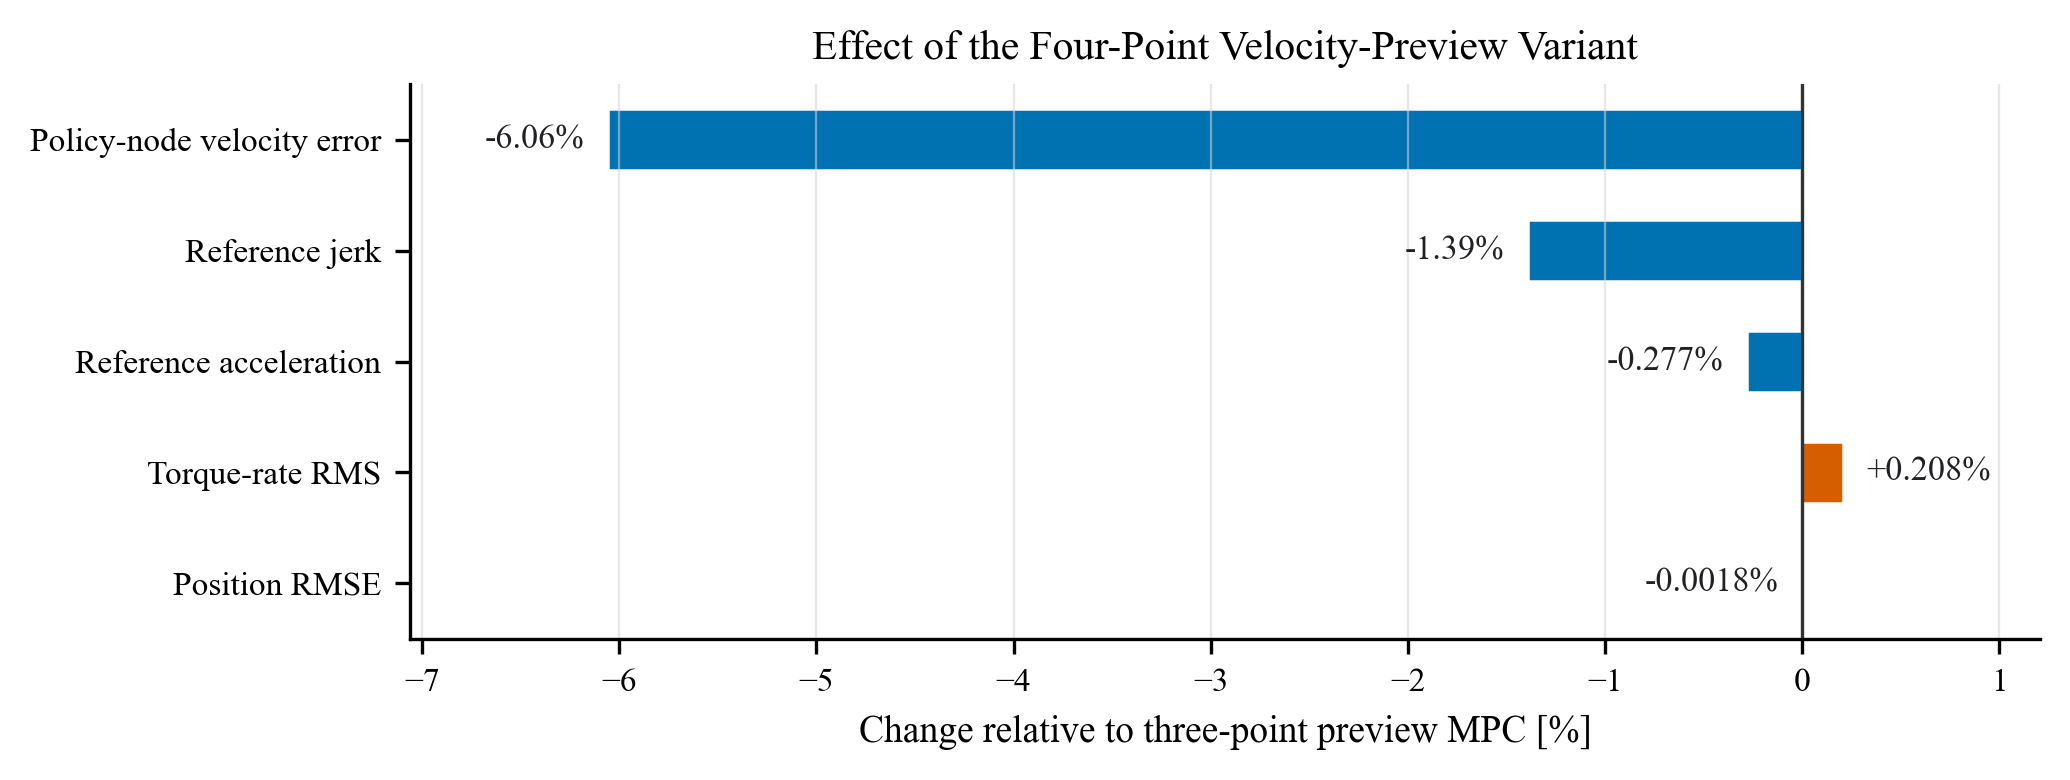
\includegraphics[width=0.92\textwidth]{mpc_velocity_variant_summary.png}
\caption{四点速度预览变体相对于三点软预览 MPC 的总体指标变化。负值表示对应 RMS 指标下降。}
\label{fig:mpc_summary}
\end{figure}

\begin{table}[htbp]
\centering
\caption{预览 MPC 对比实验的分关节指标}
\label{tab:mpc_joint}
\resizebox{\textwidth}{!}{
\begin{tabular}{llcccc}
\toprule
方法 & 关节 & 位置 RMSE & 速度 RMSE & 参考 jerk RMS & 策略点速度误差 RMS \\
\midrule
三点软预览 MPC & 右髋俯仰关节 & 0.0231147 & 0.110807 & 786.820 & 0.0842776 \\
三点软预览 MPC & 右膝 & 0.0145314 & 0.0712258 & 983.525 & 0.105347 \\
四点速度预览 & 右髋俯仰关节 & 0.0231142 & 0.110814 & 775.877 & 0.0791707 \\
四点速度预览 & 右膝 & 0.0145312 & 0.0712414 & 969.846 & 0.0989634 \\
\bottomrule
\end{tabular}}
\end{table}

分关节结果见表~\ref{tab:mpc_joint}。右髋俯仰关节与右膝在位置 RMSE 上几乎没有可解释的变化，而策略点速度误差均有下降。该现象与四点速度预览的设计目标一致：它没有改变第一个策略点位置硬约束，也没有把速度变成硬边界，而是在原有软预览框架内增加一项温和的速度一致性偏好。

\subsection{EID 输入逆的数值大小}

EID 输入逆实验使用相同的右髋俯仰关节与右膝，控制周期为 \(T_s=0.002\) s。表~\ref{tab:eid_coefficients} 给出由当前单关节模型计算得到的输入矩阵、普通伪逆和等效新增益。可以看到，输入矩阵中的速度分量约为位置分量的 \(1/T_s\) 倍，因此普通伪逆天然对速度残差非常敏感。

\begin{table}[htbp]
\centering
\caption{EID 输入矩阵、普通伪逆和输入逆等效增益}
\label{tab:eid_coefficients}
\resizebox{\textwidth}{!}{
\begin{tabular}{lcccc}
\toprule
关节 & \(J_\mathrm{eff}\) & \(g\) & \(g^+\) & \(K_u^{\mathrm{new}}=g^+K_o\) \\
\midrule
右髋俯仰关节 & 1.00508532 &
\(\begin{bmatrix}3.9798{\times}10^{-6}\\1.9899{\times}10^{-3}\end{bmatrix}\) &
\(\begin{bmatrix}1.0051 & 502.5406\end{bmatrix}\) &
\(\begin{bmatrix}0.8041 & 100.5081\end{bmatrix}\) \\
右膝 & 0.25014840 &
\(\begin{bmatrix}1.5991{\times}10^{-5}\\7.9953{\times}10^{-3}\end{bmatrix}\) &
\(\begin{bmatrix}0.2501 & 125.0737\end{bmatrix}\) &
\(\begin{bmatrix}0.2001 & 25.0147\end{bmatrix}\) \\
\bottomrule
\end{tabular}}
\end{table}

与原经验增益 \(K_u=(12,1)\) 相比，输入逆等效增益的位置通道反而更小，而速度通道显著增大。右髋俯仰关节的速度通道从 1 变为 100.5081，右膝从 1 变为 25.0147。这个结果不是调参造成的偶然现象，而是由 \(T_s/J_\mathrm{eff}\) 和 \(T_s^2/J_\mathrm{eff}\) 的尺度差异直接决定的。

\subsection{离线重放与贡献拆分}

将当前实机日志离线重放后，可以比较原经验补偿 \(K_u\eta\) 与普通伪逆估计 \(g^+K_o(x-\hat x)\) 的 RMS 大小。结果见表~\ref{tab:eid_replay}。普通伪逆估计与原补偿具有一定趋势一致性，相关系数约为 0.92，但幅值远大于当前实际补偿：右髋俯仰关节约放大 447 倍，右膝约放大 124 倍。

\begin{table}[htbp]
\centering
\caption{当前经验补偿与普通伪逆输入估计的离线重放对比}
\label{tab:eid_replay}
\begin{tabular}{lcccc}
\toprule
关节 & 当前补偿 RMS & 普通伪逆 RMS & 放大倍数 & 相关系数 \\
\midrule
右髋俯仰关节 & 0.01321 & 5.91 & 447.4 & 0.9167 \\
右膝 & 0.01842 & 2.284 & 124.0 & 0.9178 \\
\bottomrule
\end{tabular}
\end{table}

进一步拆分普通伪逆的来源可知，幅值放大几乎全部来自速度通道。右髋俯仰关节的位置项贡献仅为 \(0.00071\) N m，而速度项贡献为 \(5.91\) N m；右膝位置项贡献为 \(0.00019\) N m，速度项贡献为 \(2.28\) N m。这一结果表明，普通伪逆给出的不是对经验 \(K_u\) 的同尺度修正，而是一个对速度残差非常敏感的输入域估计。它同时会把速度残差、速度估计噪声和模型不一致性映射为较大的输入力矩；至于这一尺度是否适合闭环使用，需要结合后续实验目标和安全边界另行判断。

\subsection{EID 输入逆等效增益的闭环仿真}

为检查输入逆等效增益进入闭环后的基本趋势，在 MuJoCo 中进行 A/B 对比。两组仿真使用相同轨迹、相同观测器增益和相同控制周期，只改变输入补偿通道中的增益：基线使用 \(K_u=(12,1)\)，对比组使用表~\ref{tab:eid_coefficients} 中的 \(K_u^{\mathrm{new}}\)。需要强调的是，该实验测试的是等效新增益闭环，而不是完整的 \(g^+K_o(x-\hat x)\) 残差直注入控制器。

\begin{figure}[htbp]
\centering
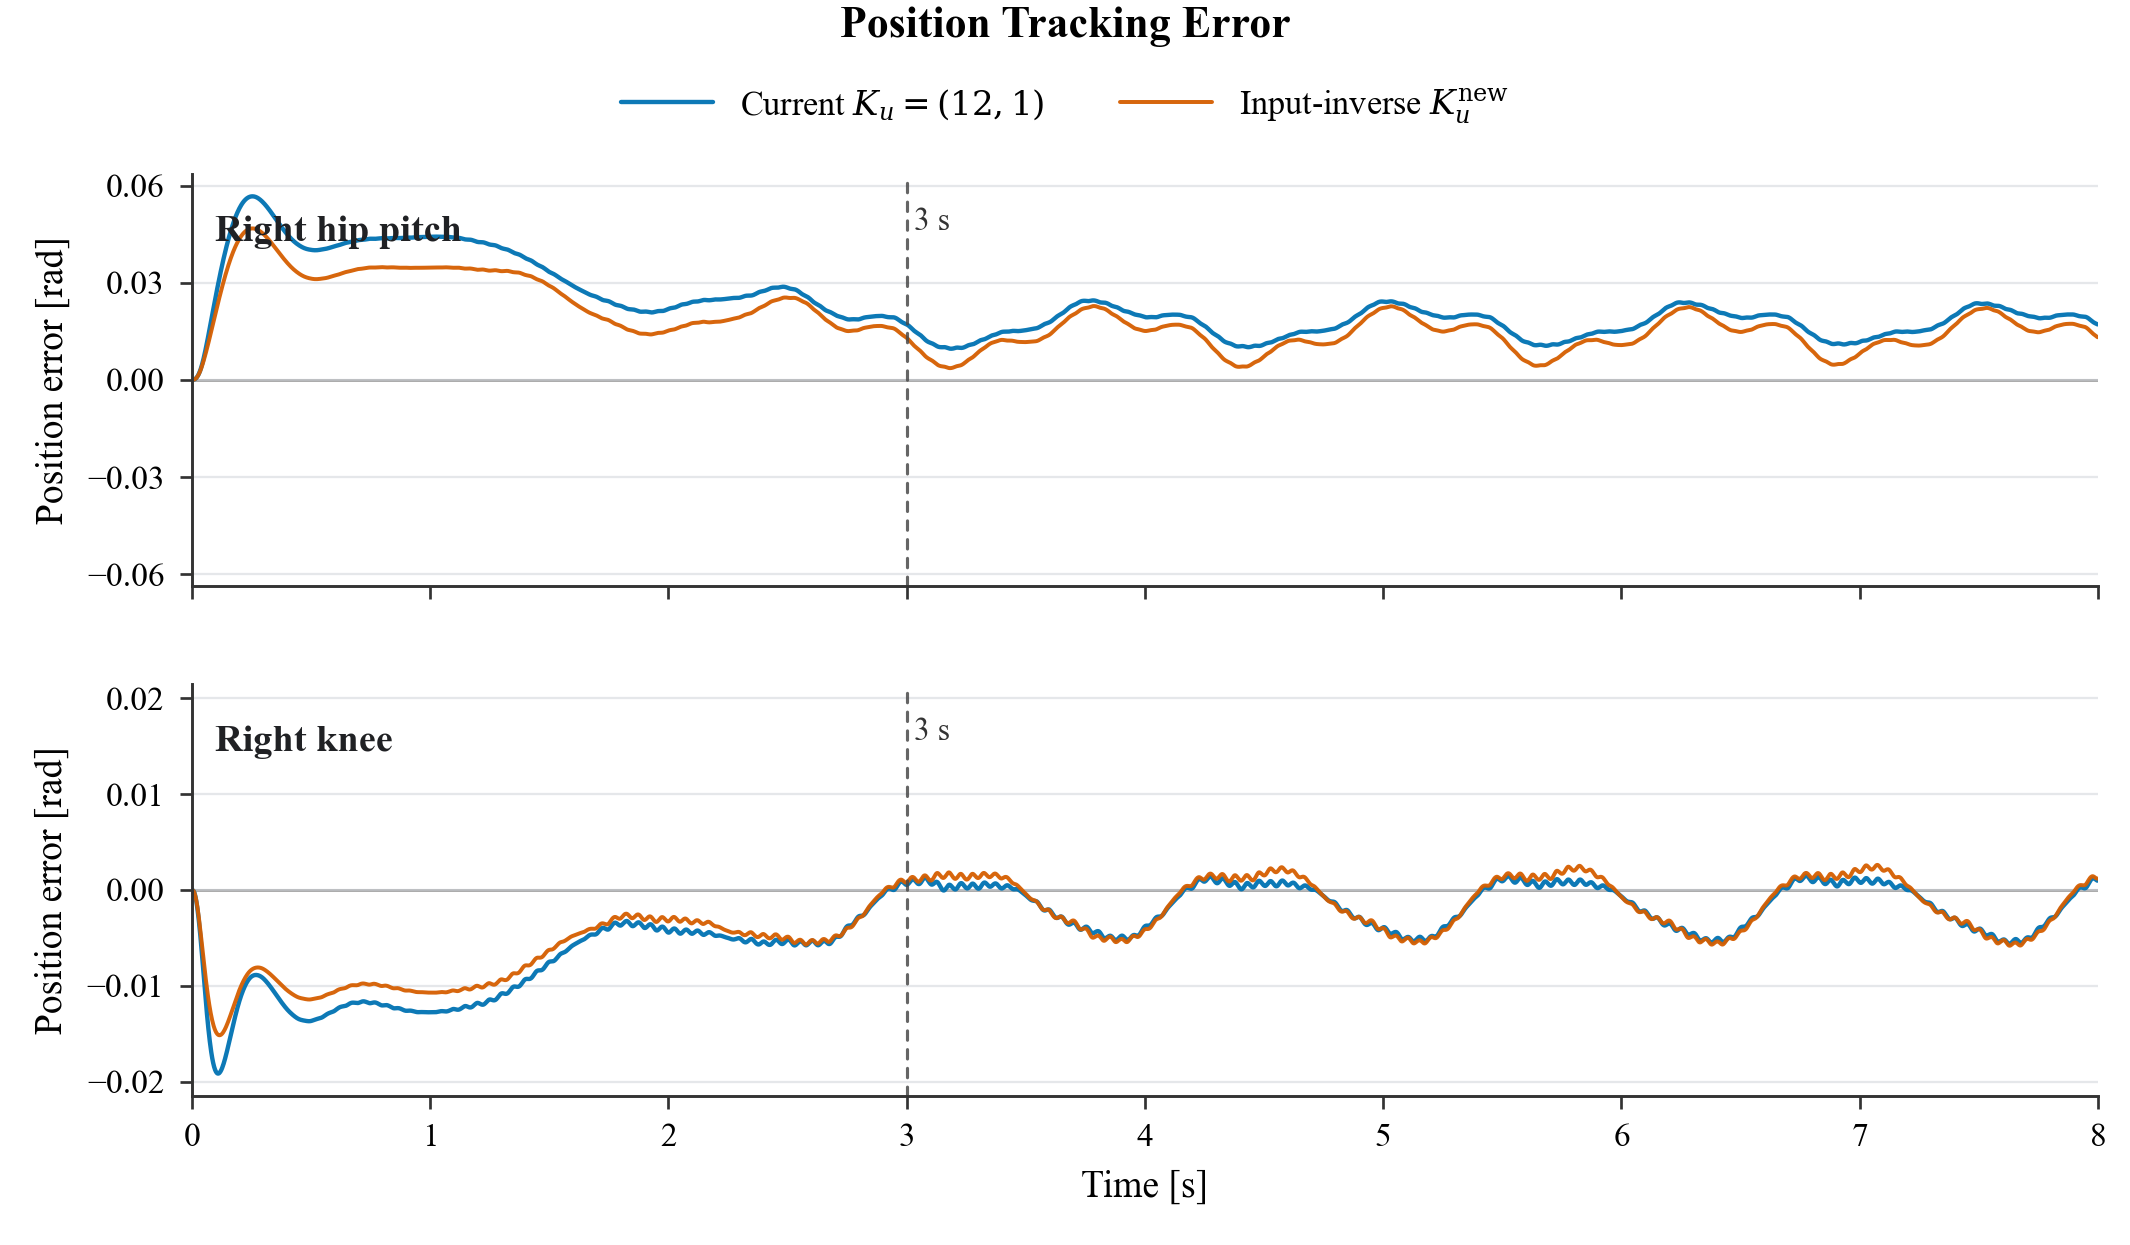
\includegraphics[width=0.95\textwidth]{eid_q_error_timeseries.png}
\caption{EID 输入逆等效增益闭环中的位置误差时间序列。曲线显示右髋俯仰关节误差有所下降，而右膝误差变化较小且略有恶化。}
\label{fig:eid_q_error}
\end{figure}

\begin{figure}[htbp]
\centering
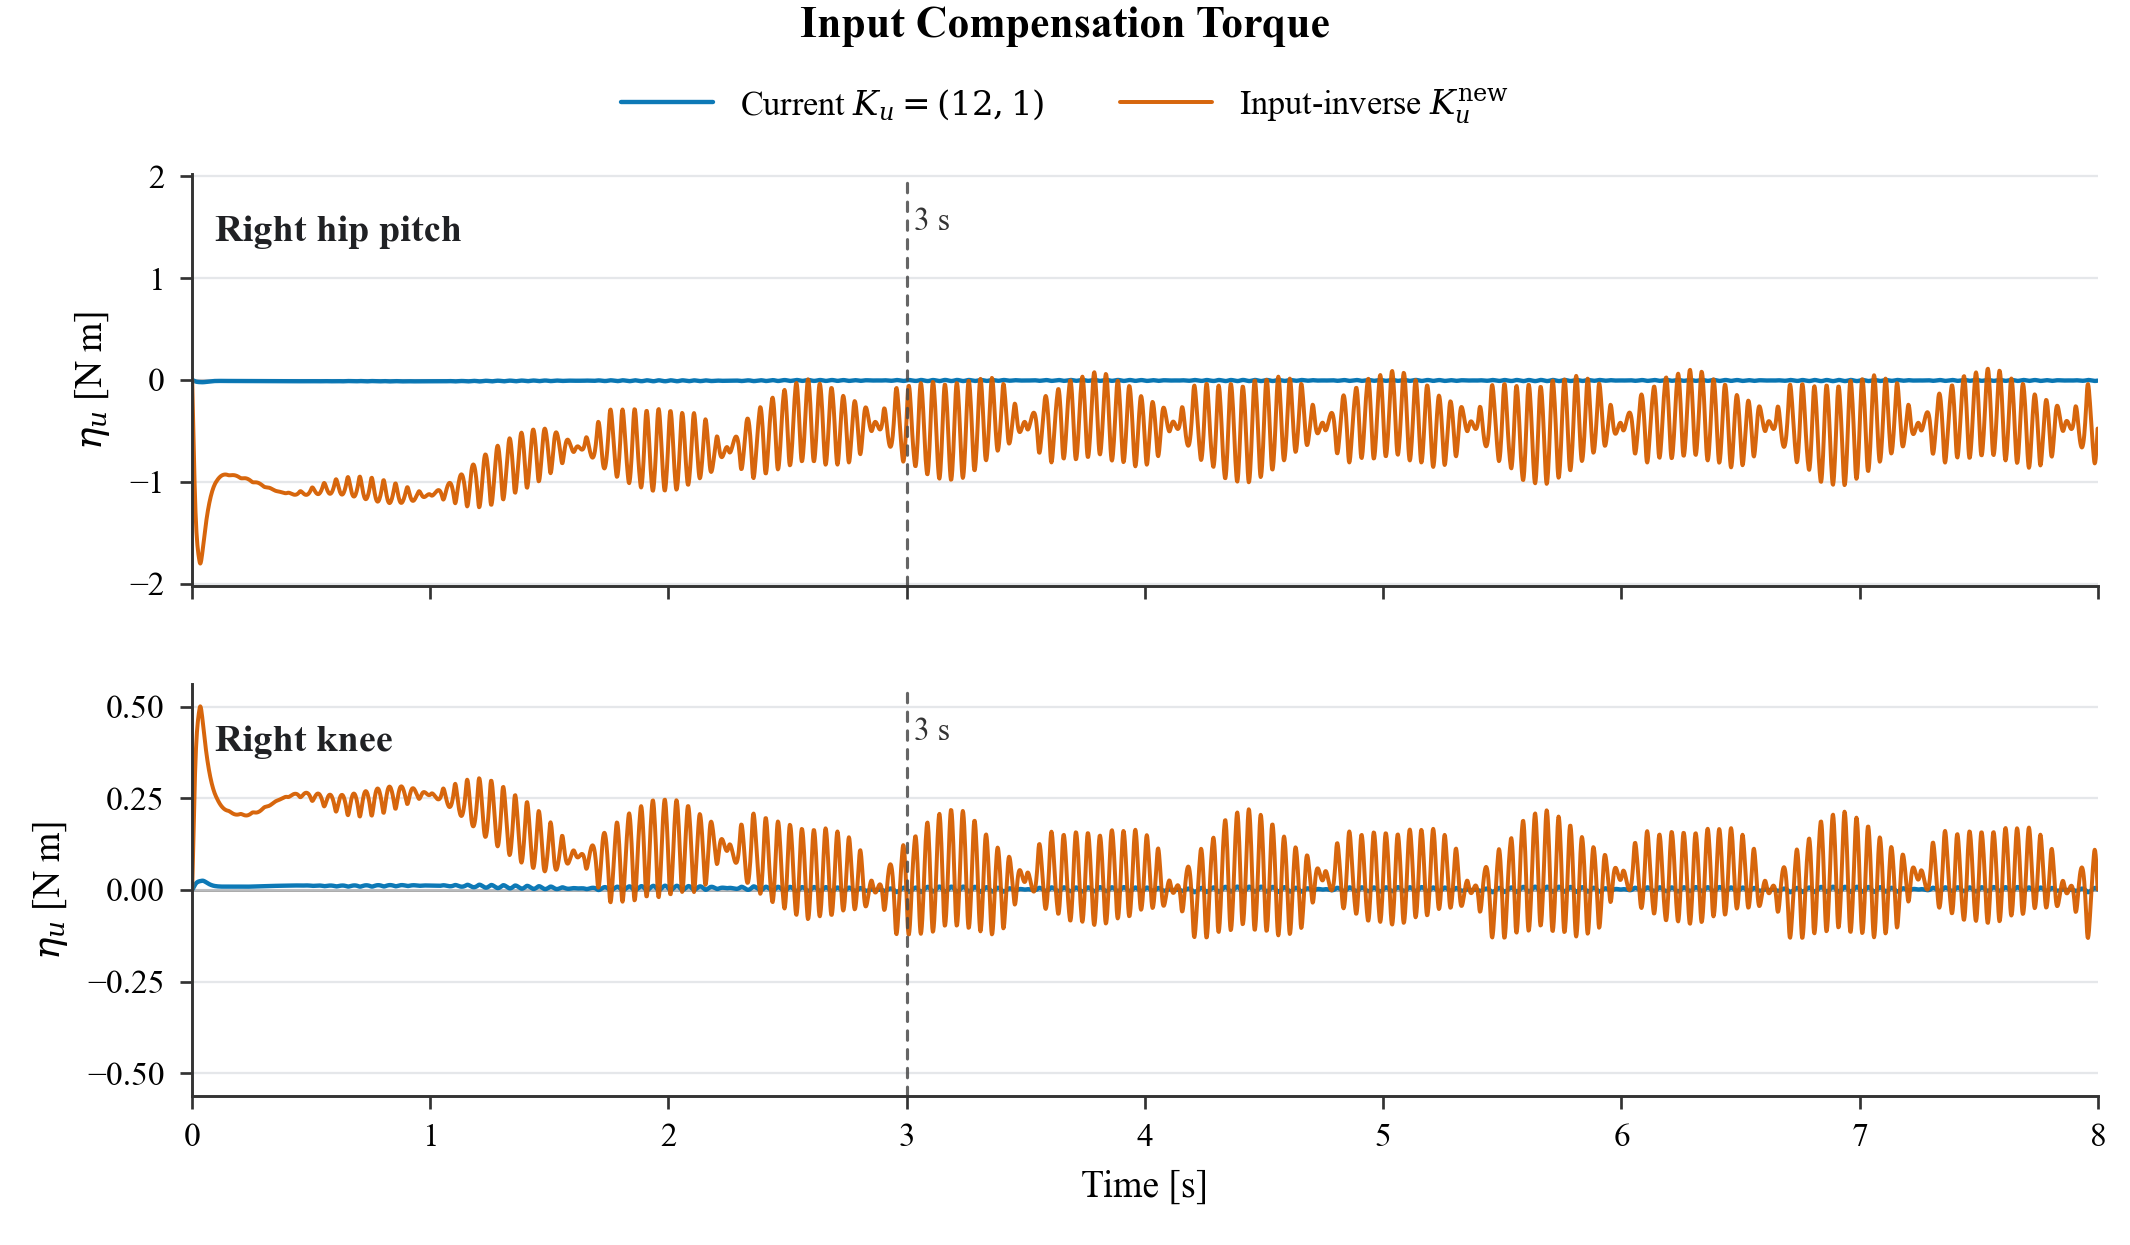
\includegraphics[width=0.95\textwidth]{eid_eta_u_timeseries.png}
\caption{EID 输入逆等效增益闭环中的输入补偿力矩时间序列。输入逆等效增益显著提高补偿幅值，尤其是在速度残差主导的右髋俯仰关节上更为明显。}
\label{fig:eid_eta_u}
\end{figure}

\begin{table}[htbp]
\centering
\caption{EID 输入逆等效增益的 MuJoCo 闭环对比}
\label{tab:eid_mujoco}
\resizebox{\textwidth}{!}{
\begin{tabular}{llcccc}
\toprule
条件 & 关节 & 位置 RMSE & 速度 RMSE & 输入补偿 RMS & 力矩 RMS \\
\midrule
原经验增益 & 右髋俯仰关节 & 0.01780 & 0.03237 & 0.005829 & 1.804 \\
原经验增益 & 右膝 & 0.002716 & 0.02570 & 0.003957 & 1.169 \\
输入逆等效增益 & 右髋俯仰关节 & 0.01462 & 0.04332 & 0.5039 & 1.821 \\
输入逆等效增益 & 右膝 & 0.002934 & 0.02641 & 0.08740 & 1.173 \\
\bottomrule
\end{tabular}}
\end{table}

表~\ref{tab:eid_mujoco} 与图~\ref{fig:eid_q_error}、图~\ref{fig:eid_eta_u} 显示，输入逆等效增益在 MuJoCo 中没有导致闭环发散。右髋俯仰关节位置 RMSE 从 0.01780 rad 降至 0.01462 rad，改善约 \(17.9\%\)；右膝位置 RMSE 从 0.002716 rad 增至 0.002934 rad，变差约 \(8.0\%\)。同时，输入补偿 RMS 明显增大：右髋俯仰关节从 0.005829 N m 增至 0.5039 N m，右膝从 0.003957 N m 增至 0.08740 N m。该结果说明输入逆等效增益确实会改变闭环行为，但收益不均匀，并伴随显著的补偿幅值放大。

\subsection{当前实机基准}

当前实机控制器在去掉前 \(3\) s 启动段后的基准跟踪误差见表~\ref{tab:hardware_baseline}。该结果说明，原控制器在当前右髋俯仰关节与右膝反相正弦跟踪实验中的误差处于正常范围。输入逆分析在本文中仅提供后续补偿结构讨论所需的模型尺度和实验参照，并不构成新的实机替换验证。

\begin{table}[htbp]
\centering
\caption{当前实机控制器的基准跟踪误差}
\label{tab:hardware_baseline}
\resizebox{\textwidth}{!}{
\begin{tabular}{lccccc}
\toprule
关节 & 位置 RMSE & 位置误差 95\% & 位置误差峰值 & 速度 RMSE & 力矩 RMS \\
\midrule
右髋俯仰关节 & 0.007733 & 0.01500 & 0.01777 & 0.1050 & 2.731 \\
右膝 & 0.01673 & 0.03054 & 0.03188 & 0.2129 & 2.532 \\
\bottomrule
\end{tabular}}
\end{table}

\section{讨论}

预览 MPC 与 EID 输入逆的实验现象具有不同含义。四点速度预览变体的效果主要体现在参考生成层。它使策略点速度误差下降约 \(6.06\%\)，并轻微降低参考加速度和 jerk，但位置 RMSE 基本不变。这说明当前三点软预览 MPC 已经能很好地满足位置节点约束；额外速度项更多是在调节节点间的速度一致性，而不是显著提高最终位置跟踪精度。由于力矩变化率略有上升，后续若继续增大速度权重，应同时观察参考加速度、jerk 和执行端力矩变化率。

EID 输入逆的现象则更偏向补偿结构的尺度分析。普通伪逆由当前离散单关节模型直接推出，形式上比经验 \(K_u\) 更接近输入矩阵几何关系；但由于采样周期很小，速度通道伪逆系数达到百级乃至五百级，导致很小的速度残差也会被映射为较大的力矩扰动。离线重放中普通伪逆 RMS 比当前补偿大两个到三个数量级，正是该尺度问题的直接体现。MuJoCo 等效增益闭环没有发散，但补偿幅值的增加和关节间收益差异说明，普通伪逆映射带来的闭环影响并不只是跟踪误差单一指标上的变化。

\section{结论}

本文将预览 MPC 参考生成与输入域 EID 补偿放在统一的髋膝关节跟踪控制框架中进行了整理。三点软预览 MPC 使用 jerk 作为决策变量，通过第一个策略点硬约束和后两个策略点软预览，在位置到达和平滑性之间取得折中。四点速度预览变体在此基础上加入由相邻策略位置差分得到的速度软目标；MuJoCo 结果显示，它主要改善策略点速度一致性并轻微降低参考 jerk，而位置跟踪误差基本不变。

EID 输入逆部分从当前半隐式欧拉单关节模型推导输入矩阵 \(g=[T_s^2/J_\mathrm{eff},\,T_s/J_\mathrm{eff}]^T\) 及其普通伪逆 \(g^+\)，并得到等效新增益 \(K_u^{\mathrm{new}}=g^+K_o\)。数值结果显示，输入逆等效增益的位置通道小于原经验增益，而速度通道显著放大。离线重放表明普通伪逆输入估计远大于当前补偿；MuJoCo 等效增益闭环中右髋俯仰关节位置误差有所改善，右膝略有恶化，同时输入补偿幅值明显增加。因此，本文的结论保持在证据范围内：四点速度预览可以继续作为参考生成候选方法评估；EID 输入逆给出了清晰的模型推导、数值尺度和实验现象，但是否以及如何进入后续闭环设计，应由后续实验约束和评价指标共同决定。

\end{document}
